
In large scale variable screening studies, we would like to find suitable designs such that combination of the dimensionality $p$, sparsity $\beta$, and signal sizes $r$ of the problem lands in the desired region of discovery, as predicted by the results in Section \ref{sec:chisq-boundaries}.

In reality, however, not all three of the parameters $(p, \beta, r)$ can be altered as we wish.
In particular, the problem dimensions and sparsity levels are usually determined by the underlying physical processes.
In the GWAS example, the number of genomic marker locations is determined by the chip used for gene sequencing, while the number of relevant genomic locations is a consequence of the biological process.
Therefore, in order to achieve a desired level of error control, we can only hope to influence the statistical signal sizes.

We discuss in this section on how to attain the necessary statistical signal sizes in the case of association tests on 2-by-2 contingency tables, and clarify the relationship between statistical signal sizes and odds ratios in such tests.

\subsection{Odds ratios and statistical power}
\label{subsec:odds-and-power}

Unlike in additive models where the parameter $\mu$ has the interpretation of signal-to-noise ratios, the meaning of the signal sizes $\lambda$ in chi-square (and other omnidirectional) tests is perhaps not as transparent.
A question frequently asked by practitioners is how this `statistical signal size' relates to odds ratios in association tests, commonly referred to as `effect size'.

Consider a 2-by-2 multinomial distribution with marginal probabilities of phenotypes $(\phi_1, \phi_2)$ and genotypes $(\theta_1, \theta_2)$.
\begin{center}
    \begin{tabular}{cccc}
    \hline
    & \multicolumn{2}{c}{Genotype} \\
    \cline{2-3}
    Probabilities & Variant 1 & Variant 2 & Total by phenotype \\
    \hline
    Cases & $\mu_{11}$ & $\mu_{12}$ & $\phi_1$ \\
    Controls & $\mu_{21}$ & $\mu_{22}$ & $\phi_2$ \\
    Total by genotype & $\theta_1$ & $\theta_2$ & 1 \\
    \hline
    \end{tabular}
\end{center}
The odds ratio is defined as the ratio of the phenotype frequencies between the two genotype variants,
\begin{equation} \label{eq:odds-ratio}
    \text{R} := \frac{\mu_{11}}{\mu_{21}}\Big/\frac{\mu_{12}}{\mu_{22}}
    = \frac{\mu_{11}\mu_{22}}{\mu_{12}\mu_{21}}.
\end{equation}
The multinomial distribution is fully parametrized by the trio $(\theta_1, \phi_1, R)$.
Odds ratios further away from 1 indicate greater contrasts between the probability of outcomes.
Independence between the genotypes and phenotyes would imply an odds ratio of zero, and hence $\mu_{jk} = \phi_j\theta_k$, for all $j,k \in\{1,2\}$.

When data are sampled from the multinomial distribution, the chi-square test defined in \eqref{eq:chisq-statistic} is asymptotically equivalent to tests including, e.g., the likelihood ratio test and Welch's t-test, both in terms of level and power \cite{ferguson2017course,gao2019upass}.

Specifically, with a sequence of local alternatives $\mu^{(1)}, \mu^{(2)}, \ldots$, such that $\sqrt{n}(\mu^{(n)}_{jk} - \phi_j\theta_k)$ converges to a constant table $\delta = (\delta_{jk})$, the aforementioned test statistics converge in distribution to the non-central chi-squared distribution with non-centrality parameter 
$\lambda = \sum_{j=1}^2 \sum_{k=1}^2 {\delta_{jk}^2}/{(\phi_j\theta_k)}$.
Hence for large samples from a fixed distribution $\mu$, the statistics would be well approximated by a $\chi^2_\nu(\lambda)$ distribution, where $\nu=1$ and
\begin{equation} 
\lambda := n\sum_{j=1}^2 \sum_{k=1}^2 \frac{(\mu_{jk} - \phi_j\theta_k)^2}{\phi_j\theta_k}.
\end{equation}
%Since $\lambda$ is linear in the number of samples $n$, 
We define 
\begin{equation} \label{eq:signal-size-chisq}
    w^2:=\lambda/n
\end{equation} 
as the \emph{signal size per sample}.
Power of association tests at $\alpha$ level is approximately $\P[\chi^2_{\nu}(\lambda)>\chi^2_{\nu,\alpha}]$, where $\chi^2_{\nu,\alpha}$ is the upper $\alpha$-quantile of a central Chi-squared distribution.
Power calculations would therefore only depend on the distributions through $\lambda=nw^2$. Statistical power would be increasing in the signal sizes per sample $w^2$.
The statistical signal size $w^2$ is jointly determined by the odds ratio (i.e., `effect size') and the marginal probabilities.

\begin{proposition} \label{prop:signal-size-odds-ratio}
Consider 2-by-2 multinomial distribution with marginals $(\phi_1, \phi_2)$ and $(\theta_1, \theta_2)$.
Let signal size $w^2$ be defined as in \eqref{eq:signal-size-chisq}, and odds ratio $\text{R}$ be defined as in \eqref{eq:odds-ratio}. 
Then we have $w^2 = 0$ if $R=1$, and
\begin{equation} \label{eq:signal-size-odds-ratio}
    w^2(\text{R}) =
    \frac{1}{4A(\text{R}-1)^2}\left(B+CR-\sqrt{(B+CR)^2-4A(R-1)^2}\right)^2,
\end{equation}
if $R\neq1$, and $R>0$, 
where $A = \phi_1\theta_1\phi_2\theta_2$, $B = \phi_1\theta_1+\phi_2\theta_2$, and $C = \phi_1\theta_2+\phi_2\theta_1$.
\end{proposition}

We illustrate Relation \eqref{eq:signal-size-odds-ratio} for selected values of marginals $\theta_1$ and $\phi_1$ in Figure \ref{fig:signal-vs-odds}.
Observe that odds ratios further away from one corresponds to stronger statistical signals per sample, ceteris paribus.
This valley pattern is in general not symmetric around 1, except for balanced marginal distributions ($\phi_1=1/2$ or $\theta_1=1/2$).
While the odds ratio $R$ can be arbitrarily close to 0 or diverge to $+\infty$ for any marginal distribution, the signal sizes $w^2$ are bounded from above by constants that depend only on the marginals.
This is quantified in the next corollary.

\begin{figure}
      \centering
      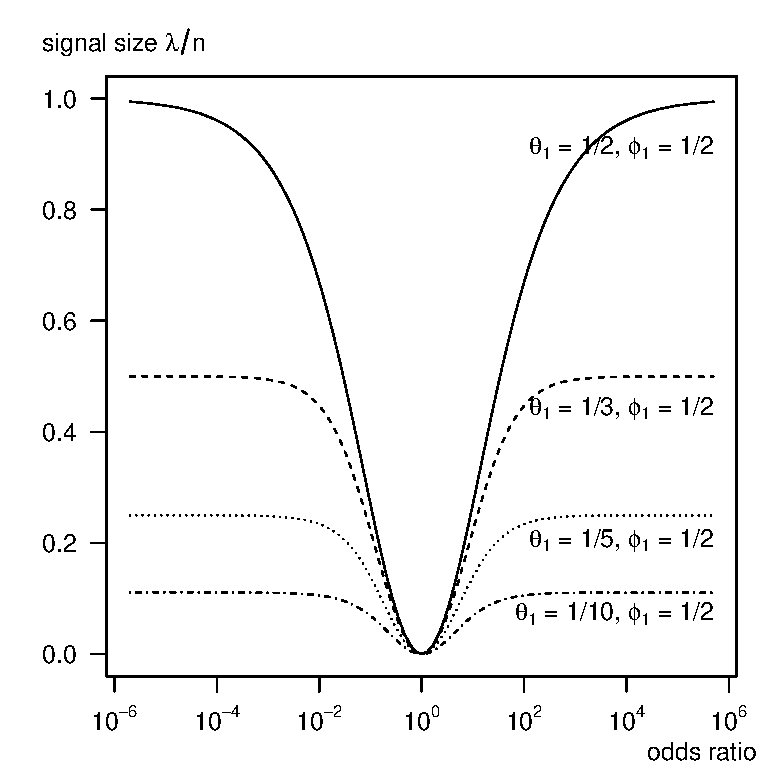
\includegraphics[width=0.49\textwidth]{./singal-vs-odds-p05}
      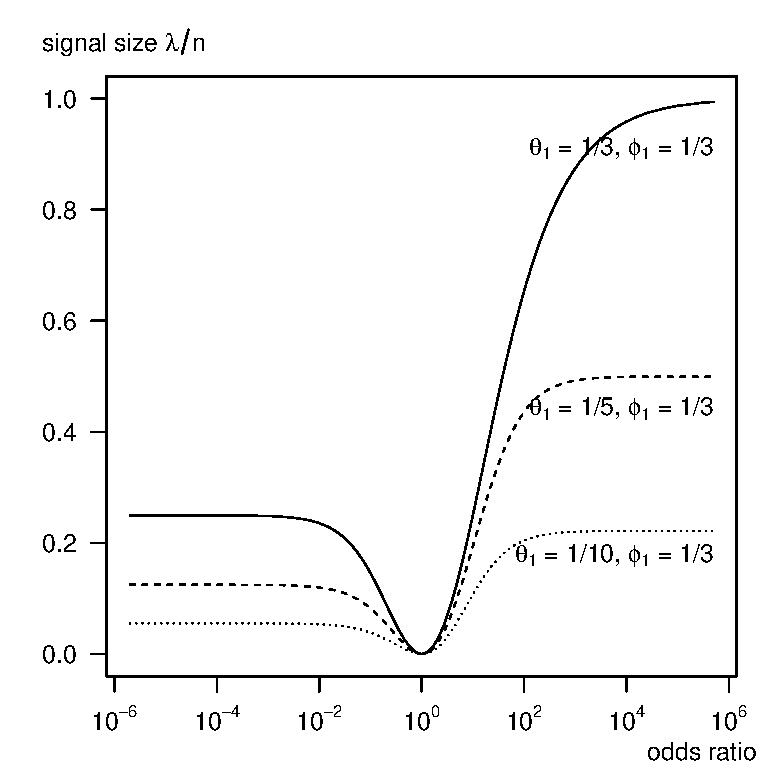
\includegraphics[width=0.49\textwidth]{./singal-vs-odds-p0333}            
      % 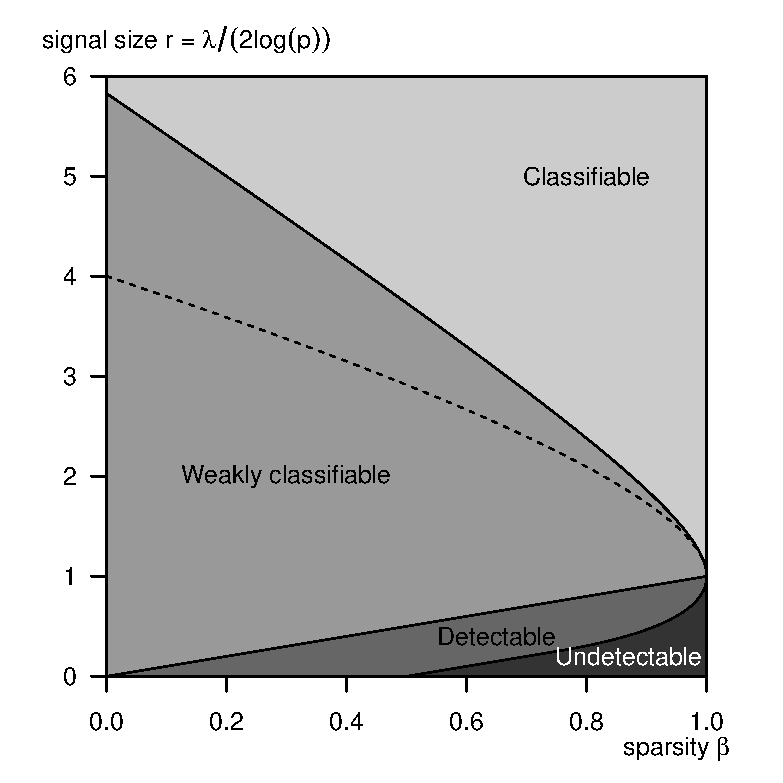
\includegraphics[width=0.35\textwidth]{./phase_diagram_chisquared.eps}
      \caption{Signal sizes per sample $w^2$ in chi-square tests as functions of odds ratios in 2-by-2 multinomial distributions, for selected marginal probabilities; see Relation \eqref{eq:signal-size-odds-ratio} in Proposition \ref{prop:signal-size-odds-ratio}.
      For fixed marginal distributions, extreme odds ratios imply stronger statistical signals at a given sample size.
      However, the signal sizes are bounded above by constants that depend on the marginal distributions; see Relations \eqref{eq:signal-size-upper-bound-1} and \eqref{eq:signal-size-upper-bound-2}.
      % Unbalanced marginal distributions -- or rare variants -- lead to smaller signal sizes at a given odds ratio.
      } 
      \label{fig:signal-vs-odds}
\end{figure}

\begin{corollary} \label{cor:signal-limits-OR}
The signal size as a function of the odds ratio $w^2(R)$ is decreasing on $(0,1)$ and increasing on $(1,\infty)$, with limits
\begin{equation} \label{eq:signal-size-upper-bound-1}
    \lim_{\text{R}\to0_+} w^2(\text{R}) = \min\left\{\frac{\phi_1\theta_1}{\phi_2\theta_2}, \frac{\phi_2\theta_2}{\phi_1\theta_1}\right\},
\end{equation}
and
\begin{equation} \label{eq:signal-size-upper-bound-2}
    \lim_{\text{R}\to+\infty} w^2(\text{R}) = \min\left\{\frac{\phi_1\theta_2}{\phi_2\theta_1}, \frac{\phi_2\theta_1}{\phi_1\theta_2}\right\}.
\end{equation}
\end{corollary}
Corollary \ref{cor:signal-limits-OR} immediately implies that balanced designs with roughly equal number of cases and controls are not necessarily the most informative.
For example, in a study where $1/3$ of the recruited subjects carrying a genetic variant that is positively correlated with the trait, a design with $1/3$ cases has $w^2$ approximately equal to 1 at large odds ratios.
This is much more efficient than a balanced design, where $w^2$ can only reach up to $1/2$; c.f., dashed curve ($\theta_1=1/3,\phi_1=1/2$) in the left panel, and solid curve ($\theta_1=1/3,\phi_1=1/3$) in the right panel of Fig. \ref{fig:signal-vs-odds}.

\subsection{Optimal study designs and rare variants}
\label{subsec:optimal-design} 

For a study with a fixed budget, that is, a fixed total number of subjects $n$ to recruit, the researcher is free to choose the fraction of cases $\phi_1$ to be included in the study.
A natural question is how the budget should be allocated to maximize the statistical power of discovery, or equivalently, one that maximizes $\lambda$ or $w^2$.


In principal, Relation \eqref{eq:signal-size-odds-ratio} can be optimized with respect to the fraction of cases $\phi_1$ in order to find optimal designs, if the rest of the parameters are known and held constant.
In practice this is not the case.
While $(\phi_1, \phi_2)$ may be controlled by by the researcher, the marginal distributions of genotypes $(\theta_1, \theta_2)$ are often unknown prior to data collection, and can change with the case-to-control ratio.

Fortunately, the conditional distributions of genotypes in the healthy control groups are often available from existing studies, and are reported in GWAS catalogs such as \cite{macarthur2016new}.
% Assume (after appropriate relabelling, hence without loss of generality) that the first variant is associated with an increased risk of disease, and is henceforth referred to as the risk variant.
We denote the conditional frequency of the first genetic variant in the control group as $(f, 1-f)$ where
$$
f := \mu_{21} / \phi_2.
$$
The multinomial distribution is fully parametrized by the conditional frequency of variant in the control group $f$, proportion of cases in the study $\phi_1$, and the odds ratio $R$.
\begin{center}
    \begin{tabular}{cccc}
    \hline
    & \multicolumn{2}{c}{Genotype} \\
    \cline{2-3}
    Probabilities & Variant 1 & Variant 2 & Total by phenotype \\
    \hline
    Cases & $\frac{\phi_1fR}{fR+1-f}$ & $\frac{\phi_1(1-f)}{fR+1-f}$ & $\phi_1$ \\
    Controls & $f(1-\phi_1)$ & $(1-f)(1-\phi_1)$ & $1-\phi_1$ \\
    \hline
    \end{tabular}
\end{center}
Proposition \ref{prop:signal-size-odds-ratio} may be re-stated in terms of the new trio $(f, \phi_1, R)$.

% Note that all these quantities refer to what is in the study, and differ from their counterparts in the general population.

\begin{corollary} \label{cor:signal-size-odds-ratio-conditional-frequency}
In the 2-by-2 multinomial distribution with marginals $(\phi_1, \phi_2 = 1-\phi_1)$, and conditional distribution of the variants in the control group $(f, 1-f)$,
Relation \eqref{eq:signal-size-odds-ratio} holds with $\theta_1 = {\phi_1fR}/{(fR+1-f)} + f(1-\phi_1)$ and $\theta_2 = 1-\theta_1$.
\end{corollary} 

The choice of $\phi_1$ now has a practical solution.

\begin{corollary} \label{cor:optimal-design}
In the context of Corollary \ref{cor:signal-size-odds-ratio-conditional-frequency},
the optimal design $(\phi^*_1, \phi^*_2)$ that maximizes the signal size per sample $w^2$ is prescribed by
\begin{equation} \label{eq:optimal-design}
    \phi_1^* = \frac{fR+1-f}{fR+1-f+\sqrt{R}}, \quad\text{and}\quad 
    \phi_2^* = 1-\phi_1^*.
\end{equation}
\end{corollary} 

Of particular interest in the genetics literature are genetic variants with very low risk alleles frequencies in the control group (i.e., $f\approx 0$), known as rare variants.
In such cases, Equation \eqref{eq:optimal-design} can be approximated by
\begin{equation} \label{eq:optimal-design-approx}
    \phi_1^* \approx \frac{1}{1 + \sqrt{R}}.
\end{equation}
For rare and adversarial mutations ($f\approx0$ and $R\gg1$), the optimal $\phi_1^*$ is close 0. 
Therefore for studies with a fixed budget $n$, controls should constitute the majority of the subjects in order to maximize power.
On the other hand for rare and protective mutations ($f\approx0$ and $R\approx0$), $\phi_1^*$ is close 1, and cases should be the majority.

\subsection{Power analysis in large scale marginal screening studies}

Returning to the problem of marginal screenings for categorical covariates, we demonstrate with an example how results in Sections \ref{sec:chisq-boundaries} and \ref{sec:signal-size-odds-ratio} can be used for planning prospective studies.

\begin{example}
In a GWAS study with $p = 10^5$ genomic marker locations\footnote{In practice, dependence among the genetic markers at different locations (known as linkage disequilibrium) decay rapidly as a function of their physical distances on the genome, the correlations of the resulting statistics are roughly independent except at short distances.}, 100 locales are believed to be associated with the trait of interest.
Specifically, these genetic variants are expected to have risk allele frequencies of $0.01$, and odds ratios of at least $1.5$.
In our parametrization of the signal sparsity \eqref{eq:signal-sparsity}, $\beta = 1 - \log(s)/\log(p) = 0.6$.

By Corollary \ref{cor:optimal-design}, the optimal design has a fraction of cases of $\phi^* = 0.478$, yielding a statistical signal size per sample of $w^2\approx9.00\time10^{-5}$ according to Proposition \ref{prop:signal-size-odds-ratio}.

If we wish to achieve family-wise error rate control, while discovering all the relevant genetic factors, Theorem \ref{thm:chi-squred-strong-boundary} predicts that the signal size $\lambda$ has to be at least $g(\beta) = \left(\sqrt{1-\beta} + \sqrt{2-\beta}\right)^2 \approx 3.30$.
This calls for a sample size of $n = \lambda / w^2 \approx 36667$, with $17527$ in the case group, and $19140$ being the controls.
\end{example}
